% answers.tex —— 1977 年·江苏镇江地区初试卷 · 参考答案与详细解析片段
% 由 tools/generate_projects.py 依来源总账自 1977/1977_数学真题_江苏镇江地区初试_试题.md + 1977/1977_数学真题_江苏镇江地区初试_解析正文.md + 1977/1977_数学真题_江苏镇江地区初试_答案要点.md 生成，勿手改（改源 MD 后重跑）


\begin{gktip}
固定源 PDF 为初试/预选卷题面扫描件，无解答可对照。以下各题均由编者独立推导，最终结论与答案要点逐题一致；原卷大题的中文数字编号已按本库规范转写为阿拉伯数字。
\end{gktip}

\begin{answer}
\gksolhead{1}{}

\textbf{题目}：

计算：

\Needspace{5\baselineskip}
（1） 

\nopagebreak[4]
\[
(-1)^4-8\times\left(-1\frac12\right)^3+20.1\div(-0.1^2).
\]

\Needspace{5\baselineskip}
（2） 

\nopagebreak[4]
\[
\frac1{2\sqrt2}-\frac{2\sqrt3}{3-\sqrt3}-\frac12\left(\sqrt{\frac12}-\sqrt{12}\right).
\]

\Needspace{5\baselineskip}
（3） 

\nopagebreak[4]
\[
\lg1-\lg0.001+\log_2(-2)^4+\log_3\sqrt3.
\]

\Needspace{5\baselineskip}
（4） 当 $a=\sqrt{10.1}$，$b=8$ 时，求式子

\nopagebreak[4]
\[
\frac{\left(a^{\frac12}b^{-1}\right)^3\sqrt{ab^{\frac23}}}{a^2b^{-4}}
\]

的值。

\Needspace{4\baselineskip}
\textbf{解析}

\gksubpart{（1）}

\nopagebreak[4]
\[
(-1)^4-8\times\left(-1\frac12\right)^3+20.1\div(-0.1^2)
=1-8\times\left(-\frac{27}{8}\right)+\frac{20.1}{-0.01}
=1+27-2010=-1982.
\]

\gksubpart{（2）}

\Needspace{5\baselineskip}
先分别有理化各项：

\nopagebreak[4]
\[
\frac1{2\sqrt2}=\frac{\sqrt2}{4},\qquad
\frac{2\sqrt3}{3-\sqrt3}=\frac{2\sqrt3(3+\sqrt3)}{(3-\sqrt3)(3+\sqrt3)}
=\frac{6\sqrt3+6}{6}=\sqrt3+1,
\]

\nopagebreak[4]
\[
\frac12\left(\sqrt{\frac12}-\sqrt{12}\right)
=\frac12\left(\frac{\sqrt2}{2}-2\sqrt3\right)
=\frac{\sqrt2}{4}-\sqrt3.
\]

\Needspace{5\baselineskip}
代入原式：

\nopagebreak[4]
\[
\frac{\sqrt2}{4}-(\sqrt3+1)-\left(\frac{\sqrt2}{4}-\sqrt3\right)
=\frac{\sqrt2}{4}-\sqrt3-1-\frac{\sqrt2}{4}+\sqrt3=-1.
\]

\gksubpart{（3）}

\Needspace{5\baselineskip}
利用 $\lg1=0$、$\lg0.001=-3$、$(-2)^4=16$、$\sqrt3=3^{\frac12}$：

\nopagebreak[4]
\[
\lg1-\lg0.001+\log_2(-2)^4+\log_3\sqrt3
=0-(-3)+\log_216+\log_33^{\frac12}
=3+4+\frac12=\frac{15}{2}.
\]

\gksubpart{（4）}

\Needspace{5\baselineskip}
先化简式子本身，与 $a$、$b$ 的具体数值无关：

\nopagebreak[4]
\[
\frac{\left(a^{\frac12}b^{-1}\right)^3\sqrt{ab^{\frac23}}}{a^2b^{-4}}
=\frac{a^{\frac32}b^{-3}\cdot a^{\frac12}b^{\frac13}}{a^2b^{-4}}
=\frac{a^{2}b^{-\frac83}}{a^2b^{-4}}
=b^{4-\frac83}=b^{\frac43}.
\]

\Needspace{5\baselineskip}
可见结果与 $a$ 无关（$a=\sqrt{10.1}$ 是多余条件）。代入 $b=8=2^3$：

\nopagebreak[4]
\[
b^{\frac43}=\left(2^3\right)^{\frac43}=2^4=16.
\]

\gkanswer{答案（1）：$-1982$。}

\gkanswer{答案（2）：$-1$。}

\gkanswer{答案（3）：$\dfrac{15}{2}$。}

\gkanswer{答案（4）：$16$。}

\end{answer}
\begin{answer}
\gksolhead{2}{}

\textbf{题目}：

（1） 求 $\sin75^\circ+\dfrac12\cos(-585^\circ)\cdot\operatorname{tg}240^\circ$ 的值。

\Needspace{5\baselineskip}
（2） 证明

\nopagebreak[4]
\[
\frac{2}{\operatorname{tg}x+\operatorname{ctg}x}=(\sin x+\cos x)^2-1.
\]

\Needspace{4\baselineskip}
\textbf{解析}

\gksubpart{（1）}

$\cos(-585^\circ)=\cos585^\circ=\cos(585^\circ-360^\circ)=\cos225^\circ=-\dfrac{\sqrt2}{2}$；

$\operatorname{tg}240^\circ=\operatorname{tg}(240^\circ-180^\circ)=\operatorname{tg}60^\circ=\sqrt3$（240° 为第三象限角，正切为正）；

$\sin75^\circ=\sin(45^\circ+30^\circ)=\sin45^\circ\cos30^\circ+\cos45^\circ\sin30^\circ=\dfrac{\sqrt6+\sqrt2}{4}$。

\Needspace{5\baselineskip}
代入：

\nopagebreak[4]
\[
\sin75^\circ+\frac12\cos(-585^\circ)\cdot\operatorname{tg}240^\circ
=\frac{\sqrt6+\sqrt2}{4}+\frac12\times\left(-\frac{\sqrt2}{2}\right)\times\sqrt3
=\frac{\sqrt6+\sqrt2}{4}-\frac{\sqrt6}{4}=\frac{\sqrt2}{4}.
\]

\gksubpart{（2）}

\nopagebreak[4]
\[
\operatorname{tg}x+\operatorname{ctg}x
=\frac{\sin x}{\cos x}+\frac{\cos x}{\sin x}
=\frac{\sin^2x+\cos^2x}{\sin x\cos x}
=\frac{1}{\sin x\cos x}.
\]

\Needspace{5\baselineskip}
所以

\nopagebreak[4]
\[
\frac{2}{\operatorname{tg}x+\operatorname{ctg}x}=2\sin x\cos x.
\]

\Needspace{5\baselineskip}
另一方面，

\nopagebreak[4]
\[
(\sin x+\cos x)^2-1=\sin^2x+2\sin x\cos x+\cos^2x-1=2\sin x\cos x.
\]

两式相等，命题得证。

\gkanswer{答案（1）：$\dfrac{\sqrt2}{4}$。}

\gkanswer{答案（2）：见解析版}

\end{answer}
\begin{answer}
\gksolhead{3}{}

\textbf{题目}：

\Needspace{5\baselineskip}
解方程

\nopagebreak[4]
\[
\frac{x-1}{x^2+4x+3}-\frac{2}{x^2-1}=0.
\]

\Needspace{4\baselineskip}
\textbf{解析}

因式分解分母：$x^2+4x+3=(x+1)(x+3)$，$x^2-1=(x-1)(x+1)$。方程定义域要求 $x\ne-1,-3,1$。

\Needspace{5\baselineskip}
原方程两边乘以公分母 $(x+1)(x+3)(x-1)$：

\nopagebreak[4]
\[
(x-1)(x-1)-2(x+3)=0
\quad\Longrightarrow\quad
x^2-2x+1-2x-6=0
\quad\Longrightarrow\quad
x^2-4x-5=0.
\]

\Needspace{5\baselineskip}
因式分解：

\nopagebreak[4]
\[
(x-5)(x+1)=0,\qquad x=5\ \text{\text{或}}\ x=-1.
\]

其中 $x=-1$ 不在定义域内（使原方程分母为零），是增根，舍去。故原方程的解为 $x=5$。

\gkanswer{答案：$x=5$。}

\end{answer}
\begin{answer}
\gksolhead{4}{}

\textbf{题目}：

求下列各函数的定义域（自变量 $x$ 的取值范围）：

（1） $y=-x+3$；

（2） $y=\dfrac1{x^2+2x-3}$；

（3） $y=\sqrt{-2x+10}$；

（4） $y=\lg(-x^2+5x-4)$。

\Needspace{4\baselineskip}
\textbf{解析}

\gksubpart{（1）}

一次函数 $y=-x+3$ 对任意实数 $x$ 都有意义，定义域为全体实数。

\gksubpart{（2）}

分式有意义要求分母不为零：$x^2+2x-3=(x+3)(x-1)\ne0$，即 $x\ne-3$ 且 $x\ne1$。

\gksubpart{（3）}

二次根式有意义要求被开方数非负：$-2x+10\ge0$，解得 $x\le5$。

\gksubpart{（4）}

对数的真数须为正：$-x^2+5x-4>0$，即 $x^2-5x+4<0$，因式分解 $(x-1)(x-4)<0$，解得 $1<x<4$。

\gkanswer{答案（1）：全体实数（$x\in\mathbb R$）。}

\gkanswer{答案（2）：$x\ne-3$ 且 $x\ne1$。}

\gkanswer{答案（3）：$x\le5$。}

\gkanswer{答案（4）：$1<x<4$。}

\end{answer}
\begin{answer}
\gksolhead{5}{}

\textbf{题目}：

从圆外一点引圆的两条割线，试证一条割线和它的圆外部分的乘积等于另一条割线和它圆外部分的乘积。

\Needspace{4\baselineskip}
\textbf{解析}

设 $P$ 为圆外一点，过 $P$ 的两条割线分别交圆于 $A$、$B$（$P$、$A$、$B$ 依次共线）和 $C$、$D$（$P$、$C$、$D$ 依次共线），求证 $PA\cdot PB=PC\cdot PD$。

\Needspace{5\baselineskip}
连结 $AC$、$BD$。因为 $A$、$C$、$D$、$B$ 四点共圆，四边形 $ACDB$ 是圆内接四边形。$\angle PAC$ 是这个圆内接四边形在顶点 $A$ 处的外角（因为 $P$、$A$、$B$ 共线，$\angle PAC=180^\circ-\angle BAC$），由“圆内接四边形的外角等于它的内对角”，

\nopagebreak[4]
\[
\angle PAC=\angle BDC.
\]

\Needspace{5\baselineskip}
又因为 $P$、$C$、$D$ 共线（$C$ 在 $P$、$D$ 之间），射线 $DC$ 与射线 $DP$ 是同一条射线，所以 $\angle BDC=\angle BDP$，从而

\nopagebreak[4]
\[
\angle PAC=\angle PDB.
\]

\Needspace{5\baselineskip}
又 $\angle APC$ 与 $\angle DPB$ 是同一个角（公共角）。于是

\nopagebreak[4]
\[
\triangle PAC\sim\triangle PDB\quad(\text{\text{两角对应相等}}).
\]

\Needspace{5\baselineskip}
由相似三角形对应边成比例，

\nopagebreak[4]
\[
\frac{PA}{PD}=\frac{PC}{PB}
\quad\Longrightarrow\quad
PA\cdot PB=PC\cdot PD.
\]

即一条割线（$PB$）与它的圆外部分（$PA$）的乘积，等于另一条割线（$PD$）与它的圆外部分（$PC$）的乘积。

\gkanswer{答案：见解析版}

\end{answer}
\begin{answer}
\gksolhead{6}{}

\textbf{题目}：

为了测量底部不能直接到达的高塔 $AB$ 的高，在地面上引一条基线 $CD=60\ \mathrm m$（$B$、$C$、$D$ 不在一直线上），今测得 $\angle ACB=30^\circ$，$\angle BCD=75^\circ$，$\angle BDC=45^\circ$，求 $AB$。
\nopagebreak[4]
\begin{center}% 1977 年江苏镇江地区初试卷第 6 题：测量不能直接到达底部的高塔 AB，
% 地面基线 CD、望塔顶 A 与塔基 B 的视线示意图（按源卷第 2 页布局）
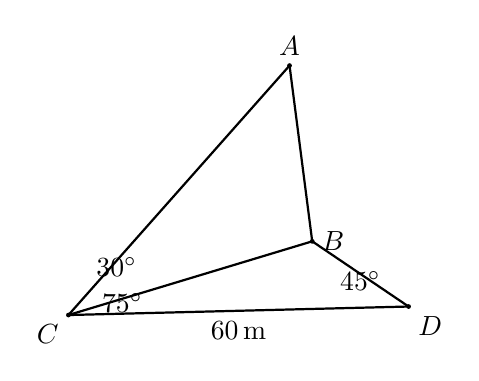
\begin{tikzpicture}[scale=0.72,>=stealth]
  \coordinate (C) at (0,0);
  \coordinate (D) at (6,0.15);
  \coordinate (B) at (4.3,1.3);
  \coordinate (A) at (3.9,4.4);
  \draw[thick] (C)--(A);
  \draw[thick] (C)--(B);
  \draw[thick] (C)--(D);
  \draw[thick] (D)--(B);
  \draw[thick] (A)--(B);
  \fill (A) circle (1.2pt) node[above] {$A$};
  \fill (B) circle (1.2pt) node[right] {$B$};
  \fill (C) circle (1.2pt) node[below left] {$C$};
  \fill (D) circle (1.2pt) node[below right] {$D$};
  \node at (0.85,0.85) {$30^\circ$};
  \node at (0.95,0.22) {$75^\circ$};
  \node at (5.15,0.6) {$45^\circ$};
  \node[below] at (3,0.05) {$60\,\mathrm{m}$};
\end{tikzpicture}
\end{center}
\nopagebreak[4]
\Needspace{4\baselineskip}
\textbf{解析}
\nopagebreak[4]
\begin{center}% 1977 年江苏镇江地区初试卷第 6 题：测量不能直接到达底部的高塔 AB，
% 地面基线 CD、望塔顶 A 与塔基 B 的视线示意图（按源卷第 2 页布局）
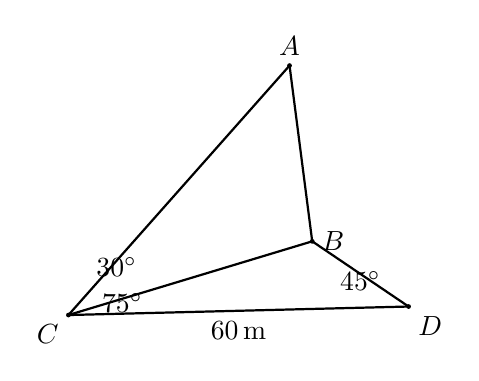
\begin{tikzpicture}[scale=0.72,>=stealth]
  \coordinate (C) at (0,0);
  \coordinate (D) at (6,0.15);
  \coordinate (B) at (4.3,1.3);
  \coordinate (A) at (3.9,4.4);
  \draw[thick] (C)--(A);
  \draw[thick] (C)--(B);
  \draw[thick] (C)--(D);
  \draw[thick] (D)--(B);
  \draw[thick] (A)--(B);
  \fill (A) circle (1.2pt) node[above] {$A$};
  \fill (B) circle (1.2pt) node[right] {$B$};
  \fill (C) circle (1.2pt) node[below left] {$C$};
  \fill (D) circle (1.2pt) node[below right] {$D$};
  \node at (0.85,0.85) {$30^\circ$};
  \node at (0.95,0.22) {$75^\circ$};
  \node at (5.15,0.6) {$45^\circ$};
  \node[below] at (3,0.05) {$60\,\mathrm{m}$};
\end{tikzpicture}
\end{center}
\nopagebreak[4]
\Needspace{5\baselineskip}
先在 $\triangle BCD$ 中求 $CB$。已知 $\angle BCD=75^\circ$，$\angle BDC=45^\circ$，故

\nopagebreak[4]
\[
\angle DBC=180^\circ-75^\circ-45^\circ=60^\circ.
\]

\Needspace{5\baselineskip}
由正弦定理，

\nopagebreak[4]
\[
\frac{CB}{\sin\angle BDC}=\frac{CD}{\sin\angle DBC}
\quad\Longrightarrow\quad
CB=\frac{CD\sin45^\circ}{\sin60^\circ}
=\frac{60\times\frac{\sqrt2}{2}}{\frac{\sqrt3}{2}}
=\frac{60\sqrt2}{\sqrt3}=20\sqrt6.
\]

\Needspace{5\baselineskip}
再在直角三角形 $ABC$（塔身 $AB$ 与地面垂直，$\angle ABC=90^\circ$）中，$\angle ACB=30^\circ$，所以

\nopagebreak[4]
\[
AB=CB\cdot\operatorname{tg}30^\circ=20\sqrt6\times\frac{1}{\sqrt3}=20\sqrt2\ (\mathrm m)\approx28.3\ \mathrm m.
\]

\gkanswer{答案：$AB=20\sqrt2\ \mathrm m\approx28.3\ \mathrm m$。}

\end{answer}
\begin{answer}
\gksolhead{7}{}

\textbf{题目}：

（1） 画出抛物线 $y=x^2+2$ 的图象，并写出它的顶点坐标、对称轴的方程和极值；

（2） 如果上述抛物线的顶点作为新的坐标原点 $O_1$，把它的对称轴作为新的纵轴 $O_1Y_1$，求这抛物线在新的直角坐标系 $X_1O_1Y_1$ 中的方程，并写出它的准线方程和焦点坐标。

\Needspace{4\baselineskip}
\textbf{解析}

\gksubpart{（1）}

$y=x^2+2$ 是开口向上的抛物线，顶点坐标为 $(0,2)$，对称轴方程为 $x=0$（即 $y$ 轴）；因开口向上，函数在 $x=0$ 处取得极小值 $2$，无极大值。

\gksubpart{（2）}

\Needspace{5\baselineskip}
以原顶点 $(0,2)$ 为新原点 $O_1$，新纵轴 $O_1Y_1$ 与原对称轴（$y$ 轴）方向一致，故坐标变换为

\nopagebreak[4]
\[
x_1=x,\qquad y_1=y-2.
\]

\Needspace{5\baselineskip}
代入 $y=x^2+2$，得 $y_1+2=x_1^2+2$，即

\nopagebreak[4]
\[
x_1^2=y_1.
\]

与标准形式 $x_1^2=4py_1$ 比较，$4p=1$，$p=\dfrac14$，故准线方程为 $y_1=-\dfrac14$，焦点坐标为 $\left(0,\dfrac14\right)$。

\gkanswer{答案（1）：顶点 $(0,2)$，对称轴 $x=0$，当 $x=0$ 时 $y$ 取极小值 $2$。}

\gkanswer{答案（2）：新坐标系中方程为 $x_1^2=y_1$，准线 $y_1=-\dfrac14$，焦点 $\left(0,\dfrac14\right)$。}

\end{answer}
\begin{answer}
\gksolhead{8}{}

\textbf{题目}：

某工厂四年来的产量，第一年到第三年的产量是按等差数列增长的，三年的总产量共 $1500$ 吨；第二年到第四年的产量是按等比数列增长的，这三年的产量共 $1820$ 吨。求每年的产量各是多少吨？

\Needspace{4\baselineskip}
\textbf{解析}

设第一、二、三年产量分别为 $a_1,a_2,a_3$（等差数列，公差 $d$），第二、三、四年产量 $a_2,a_3,a_4$ 成等比数列。

\Needspace{5\baselineskip}
由等差数列求和，

\nopagebreak[4]
\[
a_1+a_2+a_3=3a_2=1500\quad\Longrightarrow\quad a_2=500.
\]

\Needspace{5\baselineskip}
设 $a_3=500+d$（$d$ 为等差数列公差），则由等比关系 $a_4=\dfrac{a_3^2}{a_2}$，代入 $a_2+a_3+a_4=1820$：

\nopagebreak[4]
\[
500+a_3+\frac{a_3^2}{500}=1820
\quad\Longrightarrow\quad
a_3^2+500a_3-660000=0.
\]

\Needspace{5\baselineskip}
解得

\nopagebreak[4]
\[
a_3=\frac{-500+\sqrt{500^2+4\times660000}}{2}
=\frac{-500+\sqrt{2890000}}{2}
=\frac{-500+1700}{2}=600
\]

（另一根为负，舍去）。于是 $d=a_3-a_2=100$，$a_1=a_2-d=400$，$a_4=\dfrac{a_3^2}{a_2}=\dfrac{600^2}{500}=720$。

验证：$a_1,a_2,a_3=400,500,600$ 是公差 $100$ 的等差数列，和为 $1500$；$a_2,a_3,a_4=500,600,720$ 是公比 $1.2$ 的等比数列，和为 $1820$，均与题设相符。

故第一年产量 $400$ 吨，第二年 $500$ 吨，第三年 $600$ 吨，第四年 $720$ 吨。

\gkanswer{答案：第一年 $400$ 吨，第二年 $500$ 吨，第三年 $600$ 吨，第四年 $720$ 吨。}

\end{answer}
\begin{answer}
\gksolhead{9}{}

\textbf{题目}：

三角形 $ABC$ 中，$AE$ 和 $BD$ 相交于 $G$（如图），已知 $AD:DC=3:1$，$BG=GD$，求 $\dfrac{AG}{GE}$。
\nopagebreak[4]
\begin{center}% 1977 年江苏镇江地区初试卷第 9 题：三角形 ABC 中，D 在 AC 上（AD:DC=3:1），
% E 在 BC 上，AE 与 BD 相交于 G（BG=GD），按源卷第 3 页布局
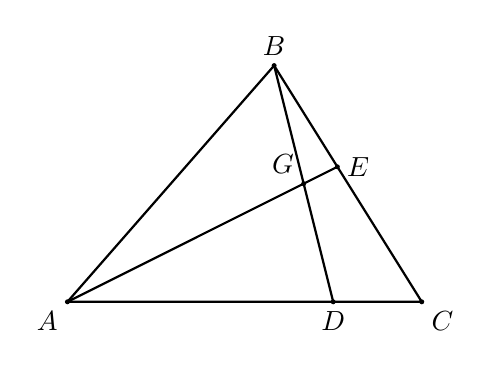
\begin{tikzpicture}[scale=0.75]
  \coordinate (A) at (0,0);
  \coordinate (C) at (6,0);
  \coordinate (B) at (3.5,4);
  \coordinate (D) at (4.5,0);
  \coordinate (E) at (4.571,2.286);
  \coordinate (G) at (4,2);
  \draw[thick] (A)--(B)--(C)--cycle;
  \draw[thick] (A)--(E);
  \draw[thick] (B)--(D);
  \fill (A) circle (1.2pt) node[below left] {$A$};
  \fill (B) circle (1.2pt) node[above] {$B$};
  \fill (C) circle (1.2pt) node[below right] {$C$};
  \fill (D) circle (1.2pt) node[below] {$D$};
  \fill (E) circle (1.2pt) node[right] {$E$};
  \fill (G) circle (1.2pt) node[above left] {$G$};
\end{tikzpicture}
\end{center}
\nopagebreak[4]
\Needspace{4\baselineskip}
\textbf{解析}
\nopagebreak[4]
\begin{center}% 1977 年江苏镇江地区初试卷第 9 题：三角形 ABC 中，D 在 AC 上（AD:DC=3:1），
% E 在 BC 上，AE 与 BD 相交于 G（BG=GD），按源卷第 3 页布局
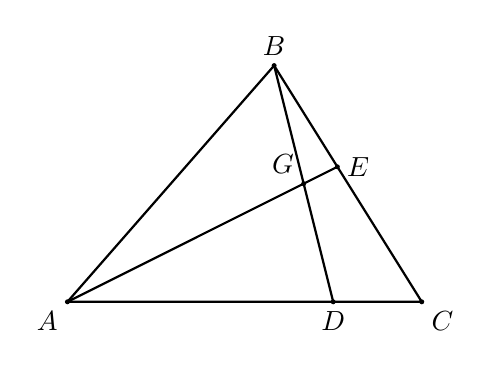
\begin{tikzpicture}[scale=0.75]
  \coordinate (A) at (0,0);
  \coordinate (C) at (6,0);
  \coordinate (B) at (3.5,4);
  \coordinate (D) at (4.5,0);
  \coordinate (E) at (4.571,2.286);
  \coordinate (G) at (4,2);
  \draw[thick] (A)--(B)--(C)--cycle;
  \draw[thick] (A)--(E);
  \draw[thick] (B)--(D);
  \fill (A) circle (1.2pt) node[below left] {$A$};
  \fill (B) circle (1.2pt) node[above] {$B$};
  \fill (C) circle (1.2pt) node[below right] {$C$};
  \fill (D) circle (1.2pt) node[below] {$D$};
  \fill (E) circle (1.2pt) node[right] {$E$};
  \fill (G) circle (1.2pt) node[above left] {$G$};
\end{tikzpicture}
\end{center}
\nopagebreak[4]
以 $A$ 为原点，记 $\vec{AB}=\boldsymbol b$，$\vec{AC}=\boldsymbol c$。

\Needspace{5\baselineskip}
因为 $AD:DC=3:1$，$D$ 在 $AC$ 上，故

\nopagebreak[4]
\[
\vec{AD}=\frac34\boldsymbol c.
\]

\Needspace{5\baselineskip}
因为 $BG=GD$，$G$ 是 $BD$ 的中点，故

\nopagebreak[4]
\[
\vec{AG}=\frac12\left(\vec{AB}+\vec{AD}\right)=\frac12\boldsymbol b+\frac38\boldsymbol c.
\]

\Needspace{5\baselineskip}
设 $E$ 在 $BC$ 上，$\vec{AE}=(1-t)\boldsymbol b+t\boldsymbol c$（$t=\dfrac{BE}{BC}$）。因为 $A$、$G$、$E$ 共线，存在常数 $s$ 使 $\vec{AG}=s\,\vec{AE}$，比较 $\boldsymbol b$、$\boldsymbol c$ 的系数（$\boldsymbol b$、$\boldsymbol c$ 不共线）：

\nopagebreak[4]
\[
s(1-t)=\frac12,\qquad st=\frac38.
\]

两式相除：$\dfrac{1-t}{t}=\dfrac{1/2}{3/8}=\dfrac43$，解得 $t=\dfrac37$；代入 $st=\dfrac38$，得 $s=\dfrac78$。

\Needspace{5\baselineskip}
于是 $\vec{AG}=\dfrac78\vec{AE}$，即 $AG:AE=7:8$，从而 $GE=AE-AG=\dfrac18AE$，故

\nopagebreak[4]
\[
\frac{AG}{GE}=\frac{7/8}{1/8}=7.
\]

\gkanswer{答案：$\dfrac{AG}{GE}=7$。}

\end{answer}